\documentclass{sigchi}

% Remove or comment out these two lines for final version
\toappearbox{Woop woop woop!}
\pagenumbering{arabic}% Arabic page numbers for submission. 

% Use \toappear{...} to override the default ACM copyright statement (e.g. for preprints).

% Load basic packages
\usepackage{balance}  % to better equalize the last page
\usepackage{graphics} % for EPS, load graphicx instead
\usepackage{times}    % comment if you want LaTeX's default font
\usepackage{url}      % llt: nicely formatted URLs

% llt: Define a global style for URLs, rather that the default one
\makeatletter
\def\url@leostyle{%
  \@ifundefined{selectfont}{\def\UrlFont{\sf}}{\def\UrlFont{\small\bf\ttfamily}}}
\makeatother
\urlstyle{leo}


% To make various LaTeX processors do the right thing with page size.
\def\pprw{8.5in}
\def\pprh{11in}
\special{papersize=\pprw,\pprh}
\setlength{\paperwidth}{\pprw}
\setlength{\paperheight}{\pprh}
\setlength{\pdfpagewidth}{\pprw}
\setlength{\pdfpageheight}{\pprh}

% Make sure hyperref comes last of your loaded packages, 
% to give it a fighting chance of not being over-written, 
% since its job is to redefine many LaTeX commands.
\usepackage[pdftex]{hyperref}
\hypersetup{
pdftitle={SIGCHI Conference Proceedings Format},
pdfauthor={LaTeX},
pdfkeywords={SIGCHI, proceedings, archival format},
bookmarksnumbered,
pdfstartview={FitH},
colorlinks,
citecolor=black,
filecolor=black,
linkcolor=black,
urlcolor=black,
breaklinks=true,
}

% create a shortcut to typeset table headings
\newcommand\tabhead[1]{\small\textbf{#1}}


% End of preamble. Here it comes the document.
\begin{document}

\title{How Does My Audience Read My Visualization?}

% Note that submissions are blind, so author information should be omitted
\numberofauthors{1}
\author{
  \alignauthor Steve Rubin\\
    \affaddr{UC Berkeley EECS, Computer Science Division}\\
    \affaddr{CS 294-10 - Visualization Class Project}\\
    \email{srubin@cs.berkeley.edu}\\
}

% Teaser figure can go here
%\teaser{
%  \centering
%  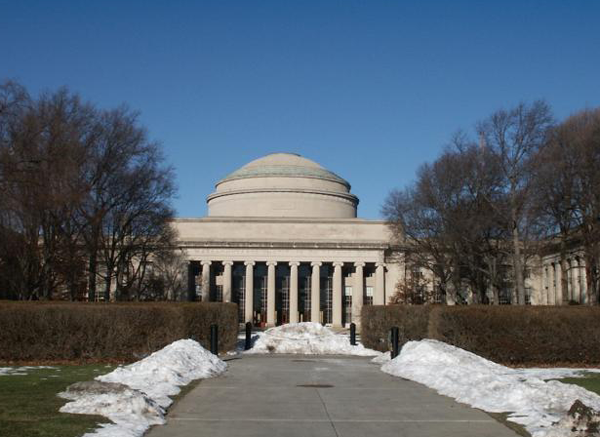
\includegraphics{Figure1}
%  \caption{Teaser Image}
%  \label{fig:teaser}
%}

\maketitle

\begin{abstract}
Abstract abstract abstract abstract.
\end{abstract}

\keywords{
  Visualization understanding; design
}

\category{H.5.m.}{Information Interfaces and Presentation (e.g. HCI)}{Miscellaneous
\\
}

\section{Introduction}

Research in information visualization and graphical perception has
often focused on creating effective visualizations for low-level
perception, such as ``what is the value represented by this bar in the
chart,'' and ``how much bigger is this bar than that bar.'' This work
is critical in gaining an understanding of which visual variables and
encodings are most easy to understand.

A parallel line of work has looked at how higher level attributes
affect the overall memorability of charts and graphs. This work aimed
to answer questions like, ``does chart junk make my graph easier to
remember,'' and ``what kinds of charts and graphs are most
memorable.''

While these two lines of work are posing interesting questions, they
neglect one of the most important goals of a visualization, which is
to convey a trend or a message to the viewer. The work on graphical
perception can tell us how to create the visualization so it is
legible, and the work on memorability can tell us how to spruce it up
so it sticks in the viewer's memory, but I am interested in learning
more about the how trends in a visualization strike a viewer as
important or unimportant. The ultimate vision of this line of research
is to take a designer's visualization, analyze it, and tell him
several key facts about the visualization, such as:

\begin{itemize}
  \item \textit{What trends do viewers think are most important?}
  \item \textit{How variable is the spread of trends that viewers
  think are important?}
  \item \textit{How well do the viewers' thoughts about this chart
  match the designer's intention?}
  \item \textit{What trends will the viewers retain after the
  visualization is taken away?}
\end{itemize}

Ideally a system could performing this analysis in a fully automated
way, but for this project we use a large amount of manual
identification and classification in the analysis pipeline in order to
illustrate the potential benefits of such a system. The final output
of this system is a dashboard that shows some of the above key facts
to the designer of the visualization.

\section{Related Work}

\subsection{Graphical Perception}

\subsection{Memory}

\subsection{Chart Junk}

\subsection{Summarization evaluation}

\section{Methods}

\subsection{Pipeline}

\subsection{Crowdsourcing}

\subsection{Nugget Analysis}

\subsection{Dashboard Generation}

\section{Results}

\section{Discussion}

\section{Future Work}

% If you want to use smaller typesetting for the reference list,
% uncomment the following line:
% \small
\bibliographystyle{acm-sigchi}
\bibliography{sample}
\end{document}
